\documentclass{beamer}

\usetheme{Warsaw}

\usepackage{amsthm}
\usepackage{verbatim}
\usepackage{xcolor}
\usepackage{listings}
\usepackage{color}
\usepackage[utf8]{inputenc}
\usepackage[T1]{fontenc}
\usepackage{textcomp}
\usepackage{graphicx} 
\usepackage[bulgarian]{babel}
\usepackage{hyperref}
\usepackage{graphicx}

\newtheorem{prob}{Задача}
\newtheorem{solv}{Решение}

\title{Въведение в Базите данни. Основни понятия и концепции.}
\author{Валентин Гелински}
\institute{ТУ София}
\date{\today} 


\begin{document}

\lstset{language=SQL,
       keywordstyle=\color{red},
       numbers=left}

  \begin{frame} 
    \titlepage
  \end{frame}

  \begin{frame}
    \frametitle{За курса}
    \begin{itemize}
      \item{Оценяване}
      \item{Курсови задачи}
    \end{itemize}
  \end{frame}

  \begin{frame}
    \frametitle{Въведение в базите данни}
    \framesubtitle{Или защо си усложняваме живота}
    \begin{itemize}
      \item{Оптимизация по обем (памет)}
      \item{Оптимизация по скорост}
      \item{Консистентност на данните}
      \item{Независимост от кода на програмата}
      \item{Сигурност}
    \end{itemize}
  \end{frame}

  \begin{frame}
    \frametitle{СУБД}
    \framesubtitle{Database Managment System}
    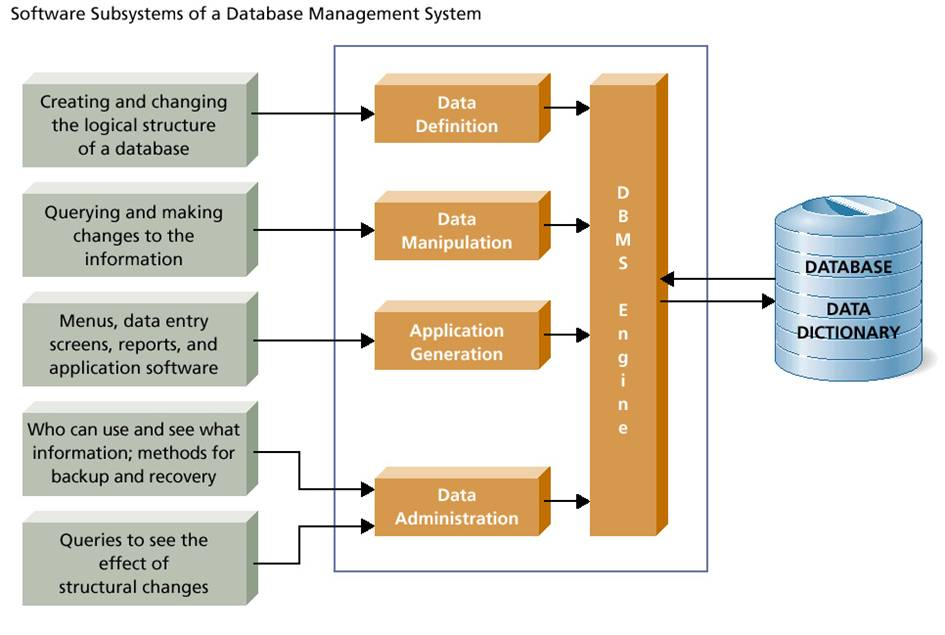
\includegraphics[width=250px]{img/rdbms}
  \end{frame}

  \begin{frame}
    \frametitle{ER model}
    \begin{itemize}
      \item{Обект}
      \item{Класове обекти}
      \item{Атрибути}
      \item{Връзки}
      \begin{itemize}
        \item{Връзки 1:1}
        \item{Връзки 1:М}
        \item{Връзки М:М}
      \end{itemize}
      \item{Характеризиращи обекти}
      \item{Подклас обекти}
    \end{itemize}
  \end{frame}

  \begin{frame}
    \frametitle{Обект}
    
\includegraphics[width=250px]{img/doge}
  \end{frame}

  \begin{frame}
    \frametitle{Клас обекти}
    \framesubtitle{Entity}
    \begin{block}{Клас обекти}
      Множество от обекти, които имат сходни и общи свойства.
    \end{block}
    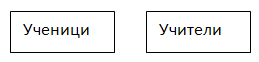
\includegraphics[width=250px]{img/entity}
  \end{frame}

  \begin{frame}
    \frametitle{Атрибут}
    \framesubtitle{Atribute}
    \begin{block}{Атрибут}
       Свойство на даден обект в даден клас
    \end{block}
    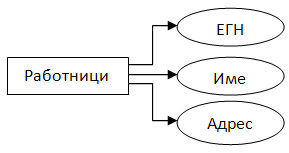
\includegraphics[width=250px]{img/atribute}
  \end{frame}

  \begin{frame}
    \frametitle{Линк}
    \framesubtitle{Relatioship}
    \begin{block}{Линк}
      Показва връзката между класовете в структурата на базата.
    \end{block}
    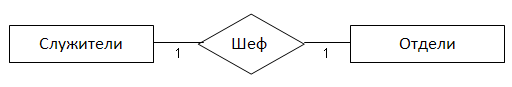
\includegraphics[width=250px]{img/relation_11}\\
    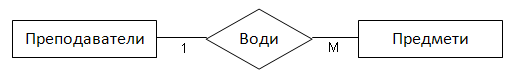
\includegraphics[width=250px]{img/relation_1m}\\
    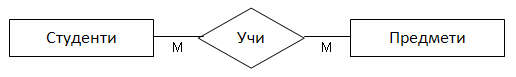
\includegraphics[width=250px]{img/relation_mm}
  \end{frame}
  
  \begin{frame}
    \frametitle{Характеризиращ обект}
    \framesubtitle{Weak entity}
    \begin{block}{Характеризиращ обект}
       Обект от предметната област, чието съществуване е невъзможно самостоятелно.
    \end{block}
    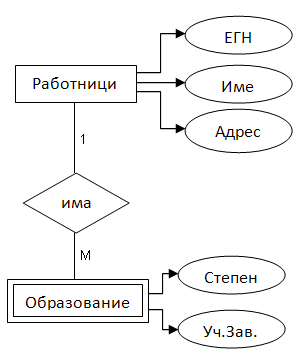
\includegraphics[width=100px]{img/weak_entity}
  \end{frame}

  \begin{frame}
    \frametitle{Подклас обекти}
    \framesubtitle{Subclass}
    \begin{block}{Подклас обекти}
      Обекти, които притежават всички свойства на даден базов клас обекти, но имат допълнителни свои атрибути.
    \end{block}
    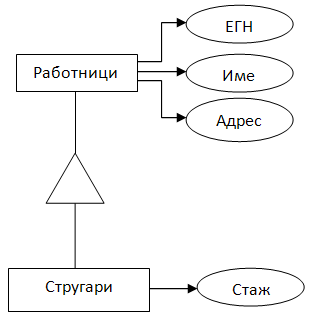
\includegraphics[width=100px]{img/subclass}
  \end{frame}

  \begin{frame}
    \frametitle{Задача}
      \begin{prob}
        Направете ER диаграма на база от данни за университети, която съдържа:\\
        - Име на университета и град в който се намира;\\
        - Номер и име на факултетите в даден университет;\\
        - Списък с преподавателите в даден факултет;\\
        - Декан на факултета;\\
        - Водени учебни предмети;\\
        - Списък със студенти, записали даден учебен предмет;\\
        - Списък на задочниците и фирмата, в която работят.
      \end{prob}
  \end{frame}


  \begin{frame}
    \frametitle{Решение}
    \begin{solv}
      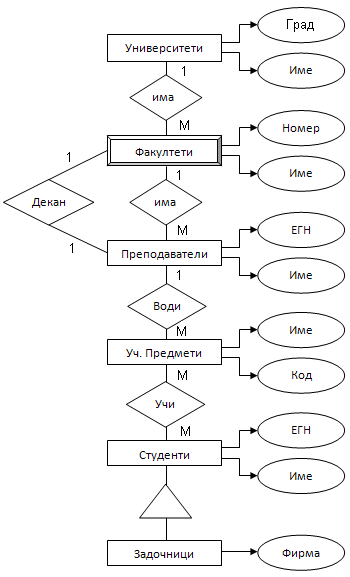
\includegraphics[width=100px]{img/problem1}
    \end{solv}
  \end{frame}

\begin{frame}[fragile]
\frametitle{Създаване на база данни}
\begin{block}{}
\begin{lstlisting}
      CREATE DATABASE <name>;
\end{lstlisting}
\end{block}
\end{frame}

\begin{frame}[fragile]
\frametitle{Създаване на таблица}
\begin{block}{}
\begin{lstlisting}
    CREATE TABLE <tablename>
    (
        <columnname> <datatype> [<other>],
        <columnname> <datatype> [<other>],
        ...
        <columnname> <datatype> [<other>]
    )
\end{lstlisting}
\end{block}
\end{frame}

\begin{frame}[fragile]
\frametitle{Пример}
\begin{block}{}
\begin{lstlisting}
	CREATE TABLE `university`.`students` (
		`firstname` TINYTEXT NOT NULL ,
		`middlename` TINYTEXT NULL ,
		`lastname` TINYTEXT NOT NULL ,
		`phone` VARCHAR( 32 ) NULL ,
		`address` TEXT NULL ,
		`faknum` BIGINT( 12 ) NOT NULL ,
		`id` INT NOT NULL AUTO_INCREMENT ,
		PRIMARY KEY ( `id` )
	) ENGINE = MYISAM ;
\end{lstlisting}
\end{block}
\end{frame}

\begin{frame}[fragile]
\frametitle{Промяна на таблици}
\begin{block}{}
\begin{lstlisting}
ALTER TABLE `university`.`zadochnici`
ADD `sruspeh` FLOAT( 3 ) NULL;

ALTER TABLE `university`.`zadochnici`
DROP `sruspeh`;

ALTER TABLE `university`.`students`
CHANGE `sruspeh` `sr_uspeh` FLOAT( 3 ) NULL;
\end{lstlisting}
\end{block}
\end{frame}
 
  
\end{document}

